\newpage

\section{Internal Software}

The in this section described processes are internal processes, i.e. running on the robot itself. In total there are three custom processes running on the robot. Figure \ref{fig:software} shows the structure of the developed software. This section focuses on the base and the navigation process. The image streaming process is referenced in section \ref{sec:image_processing}.

\begin{figure}[H]
\centering
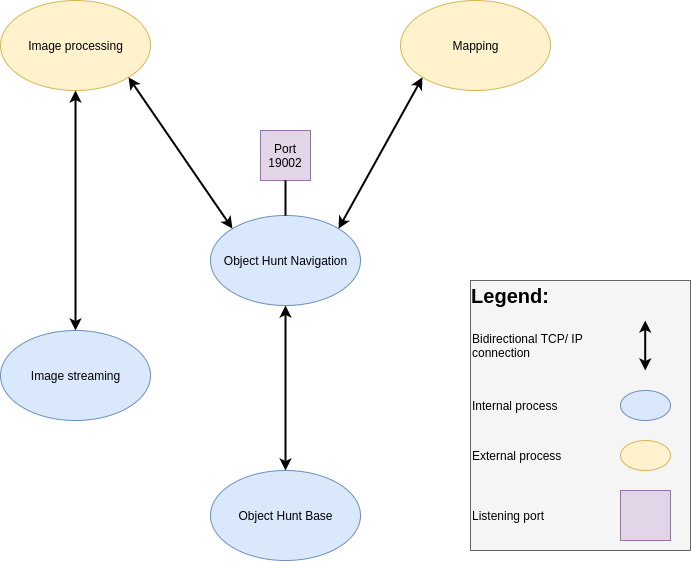
\includegraphics[scale=0.6]{sources/software_structure.png}
\caption[Software structure]{Software structure}
\label{fig:software}
\end{figure}

\subsection{Design Principles}\label{subsec:design_principles}

The system in its entirety shall not be bound to any programming language. In that way virtually any language that supports the usage of raw sockets in collaboration with TCP/\,IP can be used to develop software for the system. At the time of writing this report Java, Python and C++ are already employed.\\

Furthermore the internal software underlies particular specifications, which are defined at the beginning of the project. They define, among other things, how the system as a whole will behave and handle dedicated tasks, i.e. inter-process communication. The compliance of these principles ensure that the developed software works in the expected manner and offers the possibility for adding further processes in the future.\\

The defined principles are listed in the following:

\begin{itemize}
\itemsep0em
\item Communication
	\begin{itemize}
	\item Via TCP/\,IP
	\item Independent from other devices
	\item Beyond system border
	\end{itemize}
	
\item Economical
	\begin{itemize}
	\item No unnecessary CPU consume
	\item Fast reaction times
	\item Event driven
	\end{itemize}
	
\item Documentation
	\begin{itemize}
	\item Complete
	\item Easy accessible
	\end{itemize}
\end{itemize}

\subsubsection{Communication}

All participating processes communicate via TCP/\,IP. Therefore a purpose-built way of exchanging data is developed. Messages are generally separated in action identifiers, commands, requests and responses. Table \ref{tbl:message_definition} declares the usage of each message type.

\begingroup
\begin{tabular}[t]{|l|l|}
\hline
\makecell{Action\\identifiers} & \makecell{This messages consist of exactly one byte in all implementations. It is put in front of\\each other message type and tells the receiving process what data is about to come in.}\\
\hline
Commands & \makecell{Gives a specific order to the base process. Only the base process can handle commands.\\A command does not implicate any result, so the sending process will get no feedback,\\if the command succeeded or not.}\\
\hline
Requests & \makecell{Asks for the cars state. That can be in particular a reading of one or several sensors,\\speed or orientation data. Every request implicates a response with the desired value.\\Each request contains an identifier field.}\\
\hline
Responses & \makecell{A response message will always follow an earlier request. It can either\\indicate an invalid request or contain the desired data. Each response contains an\\identifier field. It will adopt the identifier of the respecting request.}\\
\hline
\end{tabular}
\captionof{table}{Definition of messages}\label{tbl:message_definition}
\endgroup

\newpage

There exist several implementations of each message type. A motor will most likely be controlled by a respecting command message. A sensor measurement on the other hand can be triggered by a correct request. Please refer to the project documentation page \cite{docu} for further information about which messages exist and their exact composition.

\subsubsection{Economical}

The application shall be both CPU as well as time efficient. Therefore the participating processes are implemented in a multi-threaded manner. Each thread gets created at initiation and is dedicated to one task. A thread will only be active, if the respecting task needs to executed. Otherwise the thread will be in an idle state and consume no unnecessary CPU time. Tasks are getting triggered by certain events, i.e. a hardware interrupt, an incoming message, an expired timer and so on. All events are initialized in a way that allows them to get polled from a respecting file descriptor. This allows threads and processes to wait in an idle state for specific events to happen.\\

In a multi-threaded context one has to take care of simultaneous access of shared resources. Therefore the threads are synchronized via synchronization mechanisms, i.e. mutexes. A mutex can be shared between multiple threads. If one of the threads needs to access a shared resource, it will lock the mutex. When another thread tries to access the same resource in the same time, it would need to lock the mutex as well. When the mutex is locked already, the calling thread is queued until the mutex is unlocked. As soon as the mutex gets unlocked by the initial thread, the queued thread will lock it and access the resource. In this work exclusively scoped locks are used. A scoped lock gets created whenever a mutex shall be locked. The respecting mutex is passed to the constructor of the scoped lock. The scoped lock object will be destroyed, when its scope is left and releases the mutex. This prevents a so called deadlock situation, in which a mutex is locked and cannot be unlocked anymore. A possible scenario for this is, if the locking thread experiences an error and gets stopped before unlocking the mutex.\\

The communication between different threads is realized through pipes. A pipe offers a writing as well as a reading end. Thus it allows simultaneous writing and reading by two threads without additional synchronization mechanisms. The inter-thread communication is mainly used to exchange information, trigger or abort tasks and notify each other about particular events.

\subsubsection{Documentation}

A complete and accurate documentation of the source code is produced. The software documentation tool Doxygen \cite{doxygen} is used to generate valid HTML\footnote{Hypertext Markup Language (HTML) is the standard markup language for documents designed to be displayed in a web browser} documents from annotated header files. The created files display the relations between various programming structures (classes, namespaces, etc.). Besides developers can add special denoted comments with explanatory content which are going to be adopted in the HTML files. Additional several auxiliary HTML pages with explanatory context regarding the project are created and linked to the pages created by doxygen. All created pages \cite{docu} are public accessible via the internet.\\

Moreover a Github repository \cite{github} is arranged. It contains the source code, helper scripts, mechanical construction files, schematics, PCB files, the documentation and everything else regarding this project. The data contained in the Github repository allows to rebuild the whole system developed in this work from scratch.\\

The Github repository and the online documentation are linked to each other. It is highly recommended to refer to the online resources for information about the robot as they will be kept up to date in case of changes to the system.

\newpage

\subsection{Base Process}\label{subsec:base_process}

The base process interacts directly with all controllable hardware parts listed in section \ref{sec:hardware}. Therefore it is a crucial process for the correct function of the robot. If the base process crashes unexpected, any other process concluded in the project will be disconnected or shut down as well. The base process uses only standard libraries from the C++14 standard.\\

Please see figure \ref{fig:class_diagram_base} for a simplified overview of the relations between the contained classes. Please note that the class diagram contains no exception classes for a well-arranged view.\\

\begin{figure}[H]
\centering
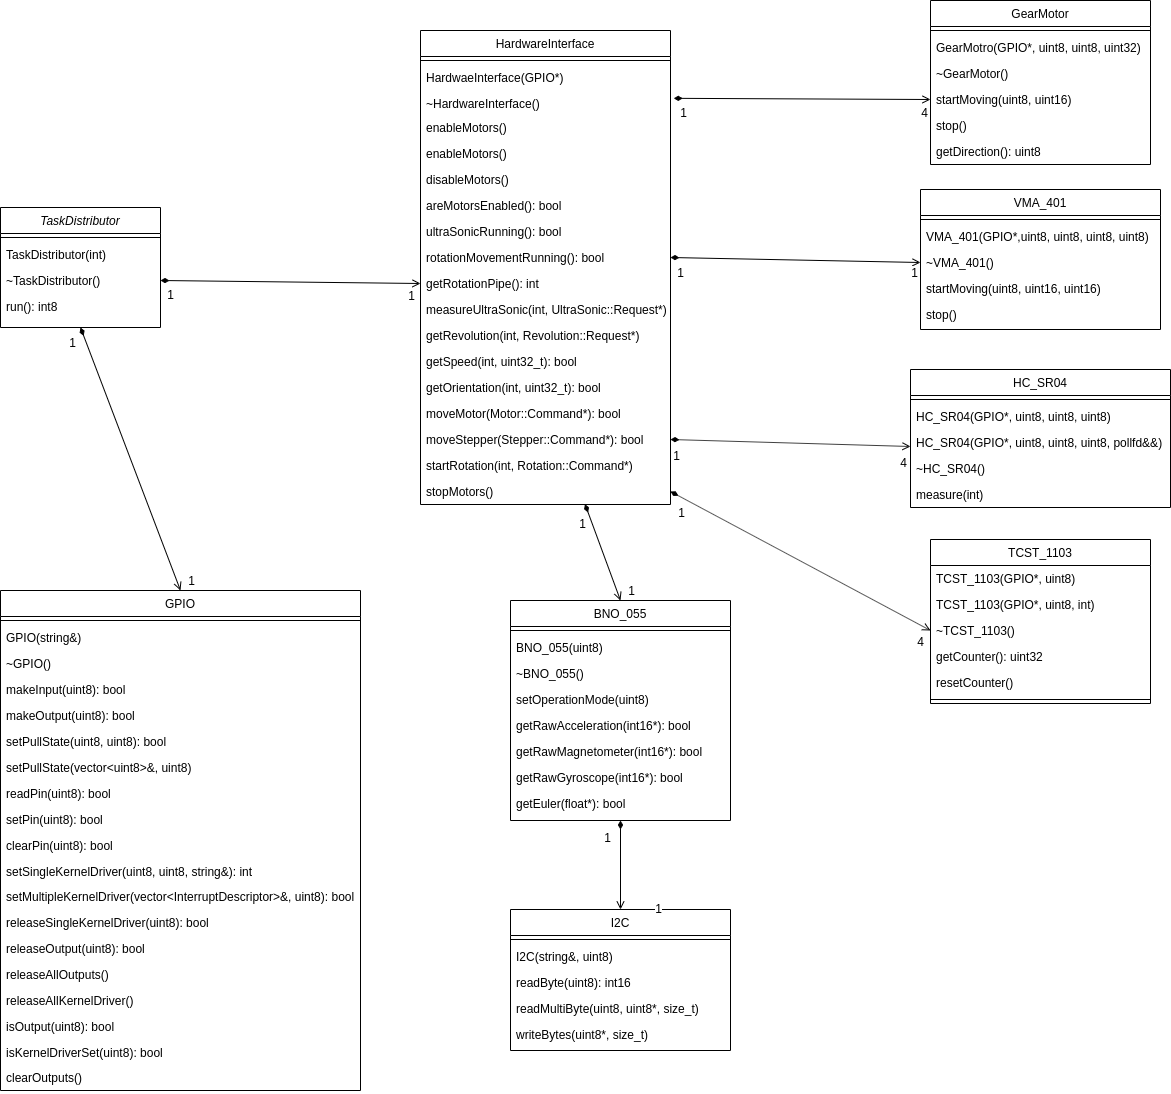
\includegraphics[width=\textwidth]{sources/class_diagram_base.png}
\caption[Class diagram base process]{Class diagram of the base process}
\label{fig:class_diagram_base}
\end{figure}

\newpage

\subsection{Navigation Process}

The navigation process establishes a connection to the base process. It requests periodical sensor readings. The responses are computed and depending on the outcome it sends movement commands to the base process. The actual movement of the robot is based on a continuous communication between both processes. The base process will stop all motors, if the navigation process experiences an error and gets shut down. The navigation process uses only standard libraries from the C++14 standard.\\
Besides the navigation process handles connections to external processes and forwards specific messages to the base process. Therefore it acts as the central point of communication between internal and external processes.\\

Please see figure \ref{fig:class_diagram_navigation} for an overview of the relations between the contained classes.

\begin{figure}[H]
\centering
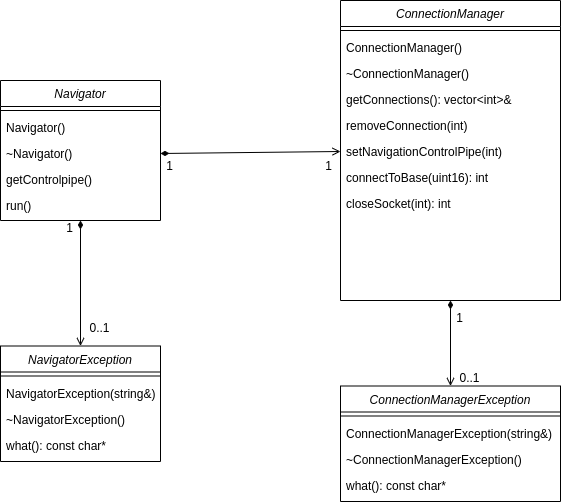
\includegraphics[width=0.8\textwidth]{sources/class_diagram_navigation.png}
\caption[Class diagram navigation process]{Class diagram of the navigation process}
\label{fig:class_diagram_navigation}
\end{figure}


